\section{Likformig rörelse}
En likformig rörelse är en rörelse som genomförs med konstant hastighet i jämvikt. Den kan egentligen sammanfattas med den så kallade ''SVT-trianglen'':
\begin{figure*}[h]
    \centering
    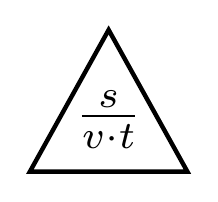
\begin{tikzpicture}[scale=2, every node/.style={scale=2}]
        \draw[ultra thick] (-0.5,-0.5) -- (0,-0.5) node[anchor=south, align=center] {\(\frac{s}{v \cdot t}\)} -- (0.5,-0.5) -- (0,0.4) -- cycle;
    \end{tikzpicture}
\end{figure*}

Denna kan användas genom att täcka för den sökta enheten med ett finger. och sedan kommer formel för den övertäcka enheten bli kvar. Sammanfattat gäller följande formler:
\begin{align*}
    s &= v \cdot t \\
    v &= \frac{s}{t} \\
    t &= \frac{s}{v} \\
\end{align*}

\section{Allmän rörelse}
All rörelse kan beskrivas med hjälp av de ovanstående formlerna men man måste blanda in lite integral- och differentialkalkyl. För att göra detta kommer man vilja uttrycka sträcka hastighet och acceleration som funktioner av tiden. Med detta menas:
\begin{equation*}
    s(t) \text{ för sträcka, } v(t) \text{ för hastighet och } a(t) \text{ för accelration.}
\end{equation*}
Denna sammanfattning antar att du kan grunderna till derivator och integraler så här är formlena anpassade för allmän rörelse:
\begin{align*}
    s(t) &= \frac{at^2}{2} + v_0t + s_0 \\
    v(t) &= s'(t) \\
    a(t) &= v'(t) = s''(t) \\[15pt]
    s(t) &=  \int{v(t)}\, dt = \iint{a(t)}\, dt
\end{align*}